%\documentclass[PhD]{iitmdiss}
%\documentclass[MS]{iitmdiss}
\documentclass[MTech]{iitmdiss}
%\documentclass[BTech]{iitmdiss}
\usepackage{times}
 \usepackage{t1enc}

\usepackage{graphicx}
\usepackage{epstopdf}
%\usepackage[hypertex]{hyperref} % hyperlinks for references.
\usepackage[driverfallback=dvipdfm]{hyperref}
\usepackage{amsmath} % easier math formulae, align, subequations \ldots

\def\thesistitle{Analysis of Parallel Incremental/Decremental Graph Colouring on GPU}
\def\thesisauthor{Mohammed Shamil}

\begin{document}


%%%%%%%%%%%%%%%%%%%%%%%%%%%%%%%%%%%%%%%%%%%%%%%%%%%%%%%%%%%%%%%%%%%%%%
% Title page

\title{\thesistitle}

\author{\thesisauthor}

\date{MAY 2016}
\department{COMPUTER SCIENCE AND ENGINEERING}

%\nocite{*}
\maketitle

%%%%%%%%%%%%%%%%%%%%%%%%%%%%%%%%%%%%%%%%%%%%%%%%%%%%%%%%%%%%%%%%%%%%%%
% Certificate
\certificate

\vspace*{0.5in}

\noindent This is to certify that the thesis titled {\bf {\thesistitle}}, submitted by {\bf {\thesisauthor}}, 
  to the Indian Institute of Technology, Madras, for
the award of the degree of {\bf Master of Technology}, is a bona fide
record of the research work done by him under our supervision.  The
contents of this thesis, in full or in parts, have not been submitted
to any other Institute or University for the award of any degree or
diploma.

\vspace*{1.5in}
\hspace*{-0.25in}
\begin{singlespace}
\noindent {\bf Dr. Rupesh Nasre} \\
\noindent Research Guide \\ 
\noindent Assistant Professor \\
\noindent Dept. of Computer Science and Engineering\\
\noindent IIT Madras, 600 036 \\
\end{singlespace}
\vspace*{0.25in}
\noindent Place: Chennai\\ 
Date: 11 May, 2016


%%%%%%%%%%%%%%%%%%%%%%%%%%%%%%%%%%%%%%%%%%%%%%%%%%%%%%%%%%%%%%%%%%%%%%
% Acknowledgements
\acknowledgements

Thanks to all those who made \TeX\ and \LaTeX\ what it is today.

%%%%%%%%%%%%%%%%%%%%%%%%%%%%%%%%%%%%%%%%%%%%%%%%%%%%%%%%%%%%%%%%%%%%%%
% Abstract

\abstract

\noindent KEYWORDS: \hspace*{0.5em} \parbox[t]{4.4in}{Colour Quality; Compressed Sparse Row Representation; Decremental Graph Colouring; GPGPU; Graph Colouring; Incremental Graph Colouring; NP-hard; nVIDIA Cuda; Parallel Computing; Parallel Graph Algorithms; Vertex Colouring.}

\vspace*{24pt}

\noindent Graphs are a well studied and widely used data structure in the field of algorithms, programming and computing. There are a lot of interesting applications of graphs and various algorithms are built on top of the graph data structure. One of the most famous and well studied graph problems is that of graph colouring. There are a lot of different versions of graph colouring problem of which the most common ones are that of vertex colouring and edge colouring. The problem is seemingly simple, to allocate a colour to every vertex/edge of a graph so that adjacent vertices/edges don't share the same colour minimizing the number of colours used.  
Graph colouring is a very important and yet very challenging graph problem with ongoing active research. Graph colouring finds application in a varied range of problems including various scheduling problems like job scheduling on distributed computing systems, register allocation in compilers, pattern matching problems and solving Sudoku boards.

Though the problem is seemingly simple, it is computationally hard. The graph colouring problem we are exploring in this work, that of vertex colouring, is an NP-hard problem. The sequential approaches like greedy colouring are simply not fast enough whereas advanced approximate/randomized solutions either produce colourings of bad colour quality or aren't fast enough. Thus came the parallel approaches to Graph Colouring. Most of the parallel versions of Graph Colouring algorithms were designed with either multi-core CPUs or heavy duty super computers in mind. With the advent of General-Purpose computing on GPUs (GPGPU), we have access to cheap heavy multi-threaded parallel computing power. Our work is based on parallel computing on nVidia GPUs using Cuda programming language.

We explore different parallel graph colouring algorithms on nVIdia GPUs in this work and try to adapt them to support addition of edges, called incremental graph colouring, and deletion of edges, called decremental graph colouring. In the first section, we explore different parallel graph algorithms and adapt a couple of them, one based on \textit{speculation} and \textit{conflict resolution} and the other on \textit{Vertex Independent Sets}, to work on nVidia GPUs. In the following sections, we adapt the GPU parallel colouring algorithm to support additions and deletions of edges. In the incremental part, we explore different methods to maximize parallelization while colouring newly added edges and use propagation to improve overall colour quality. In the decremental part, we explore different options to either process the vertices, on which the deleted edges were incident, on the go or to process them together and use propagation to propagate the information across the graph improving the colour quality.  

\pagebreak

%%%%%%%%%%%%%%%%%%%%%%%%%%%%%%%%%%%%%%%%%%%%%%%%%%%%%%%%%%%%%%%%%
% Table of contents etc.

\begin{singlespace}
\tableofcontents
\thispagestyle{empty}

\listoftables
\addcontentsline{toc}{chapter}{LIST OF TABLES}
\listoffigures
\addcontentsline{toc}{chapter}{LIST OF FIGURES}
\end{singlespace}


%%%%%%%%%%%%%%%%%%%%%%%%%%%%%%%%%%%%%%%%%%%%%%%%%%%%%%%%%%%%%%%%%%%%%%
% Abbreviations
\abbreviations

\noindent 
\begin{tabbing}
xxxxxxxxxxx \= xxxxxxxxxxxxxxxxxxxxxxxxxxxxxxxxxxxxxxxxxxxxxxxx \kill
\textbf{IITM}   \> Indian Institute of Technology, Madras \\
\textbf{RTFM} \> Read the Fine Manual \\
\textbf{GPU} \> Graphics Processing Unit \\
\textbf{GPGPU} \> General-Purpose computing on Graphics Processing Units  \\
\textbf{CSR} \> Compressed Sparse Row \\

\end{tabbing}

\pagebreak

%%%%%%%%%%%%%%%%%%%%%%%%%%%%%%%%%%%%%%%%%%%%%%%%%%%%%%%%%%%%%%%%%%%%%%
% Notation

%\chapter*{\centerline{NOTATION}}
%\addcontentsline{toc}{chapter}{NOTATION}
%
%\begin{singlespace}
%\begin{tabbing}
%xxxxxxxxxxx \= xxxxxxxxxxxxxxxxxxxxxxxxxxxxxxxxxxxxxxxxxxxxxxxx \kill
%\textbf{$r$}  \> Radius, $m$ \\
%\textbf{$\alpha$}  \> Angle of thesis in degrees \\
%\textbf{$\beta$}   \> Flight path in degrees \\
%\end{tabbing}
%\end{singlespace}
%
%\pagebreak
\clearpage

% The main text will follow from this point so set the page numbering
% to arabic from here on.


\pagenumbering{arabic}
%%%%%%%%%%%%%%%%%%%%%%%%%%%%%%%%%%%%%%%%%%%%%%%%%%
% Introduction.


\chapter{INTRODUCTION}
\label{chap:intro}
\section{Graphs and Graph Algorithms}
Graphs are really important mathematical concepts and in the area of computing, their various forms are widely used as data structures to aid various algorithms. Graphs are commonly used to denote relations between different entities and hence is a very important and integral part of many algorithms. On a practical level, we deal with graphs in the order of billions of nodes and edges on a daily basis. Especially with the advent of social networks and big data, a lot of active research is ongoing in the analysis and understanding of large graphs.

Many problems in the area of Computer Science, Biology etc. are solved with the help of algorithms which are based on graphs. Shortest path problem, Traveling Salesman Problem (TSP), network flow problems, vertex cover problem, graph colouring etc. are important graph-based problems with many practical applications in the real world. Our work is on Graph Colouring which is one of the most famous and well studied graph problems.
\section{Vertex Colouring}
Graph Colouring problem entails \textit{colouring/labeling} of the vertices/edges of a graph based on some set of conditions which are to be satisfied. In other words, its a problem in which you allocate a colour/number to every vertex/edge of a graph such that a set of constraints are satified. There are different versions of Graph Colouring and the one which is of interest to us is that of Vertex Colouring.
\subsection{Classical Vertex Colouring Problem}
Vertex Colouring is the most basic version of Graph Colouring and other Graph Colouring problems can be presented as a Vertex Colouring problem. In it's classical form, Vertex Colouring is:
\begin{verse}
\textit{\textbf{Vertex Colouring:} Colouring all the vertices of a graph such that adjacent vertices have different colours. That is, there shouldn't be an edge where the incident vertices share the same colour.}
\end{verse}
There are other forms of vertex colouring where additional conditions than the one given above need to be considered while colouring. In our work, we are concerned only with the classical form of vertex colouring which hereinafter interchangeably referred to simply as Graph Colouring.
\subsection{Chromatic Number $ \chi(G) $}
A graph \textit{G} is said to \textit{k-}colourable, if \textit{G} can be coloured using \textit{k} colours. For example, from the \textit{Four Colour Theorem}, we have that all planar graphs are 4-colourable. Also, all bipartite graphs are 2-colourable.
 
The \textit{Chromatic Number} of a graph G, denoted by $ \chi(G) $, is the minimum number of colours required to colour a graph. That is, $ \chi(G) $, is the minimum value of all \textit{k} for which the graph \textit{G} is \textit{k-}colourable. Therefore, if a graph is \textit{k-}colourable, we have:
\begin{center}
$ \chi(G) \leq k $
\end{center}
\subsection{Colour Quality}
Colour Quality is a term used to denote how good the colouring done by a particular algorithm is. Colour Quality is said to be better for an algorithm if the number of colours used by the algorithm to colour a graph \textit{G} is closer to its Chromatic Number, $\chi(G)$.

Mathematically, Colour Quality of a colouring is said to be better as the fraction,
\begin{center}
$\frac{No. \: of \: colours \: used \: by \: the \: algorithm}{\chi(G)} $
\end{center}
is closer to 1.
\subsection{Complexity}
Graph Colouring is a computationally complex problem. To decide if a Graph can be coloured using \textit{k} colours, is an NP-complete problem. Whereas, finding the Chromatic Number of a graph ($ \chi(G) $) is proved to be an NP-hard problem.

There exist many algorithms like Greedy Colouring, approximation algorithms and randomized algorithms. There also exist polynomial time algorithms for some specific family of graphs. For example, it can be decided if a graph can be coloured using 2 colours by checking if it is a bipartite graph. This can be done in polynomial time using Breadth First Search (BFS).
\subsection{Applications}
Graph Colouring problem, which started as a map colouring problem (four colour theorem), finds many important real applications including but not limited to:
\begin{itemize}
\item Scheduling problems like job scheduling across multiple nodes in a distributed computing environment
\item Register allocation problem during compilation
\item Solving Sudoku
\item Pattern matching applications
\end{itemize}
\section{Parallelization}
\subsection{Frequency Scaling}
\begin{figure}[h]
    \centering
    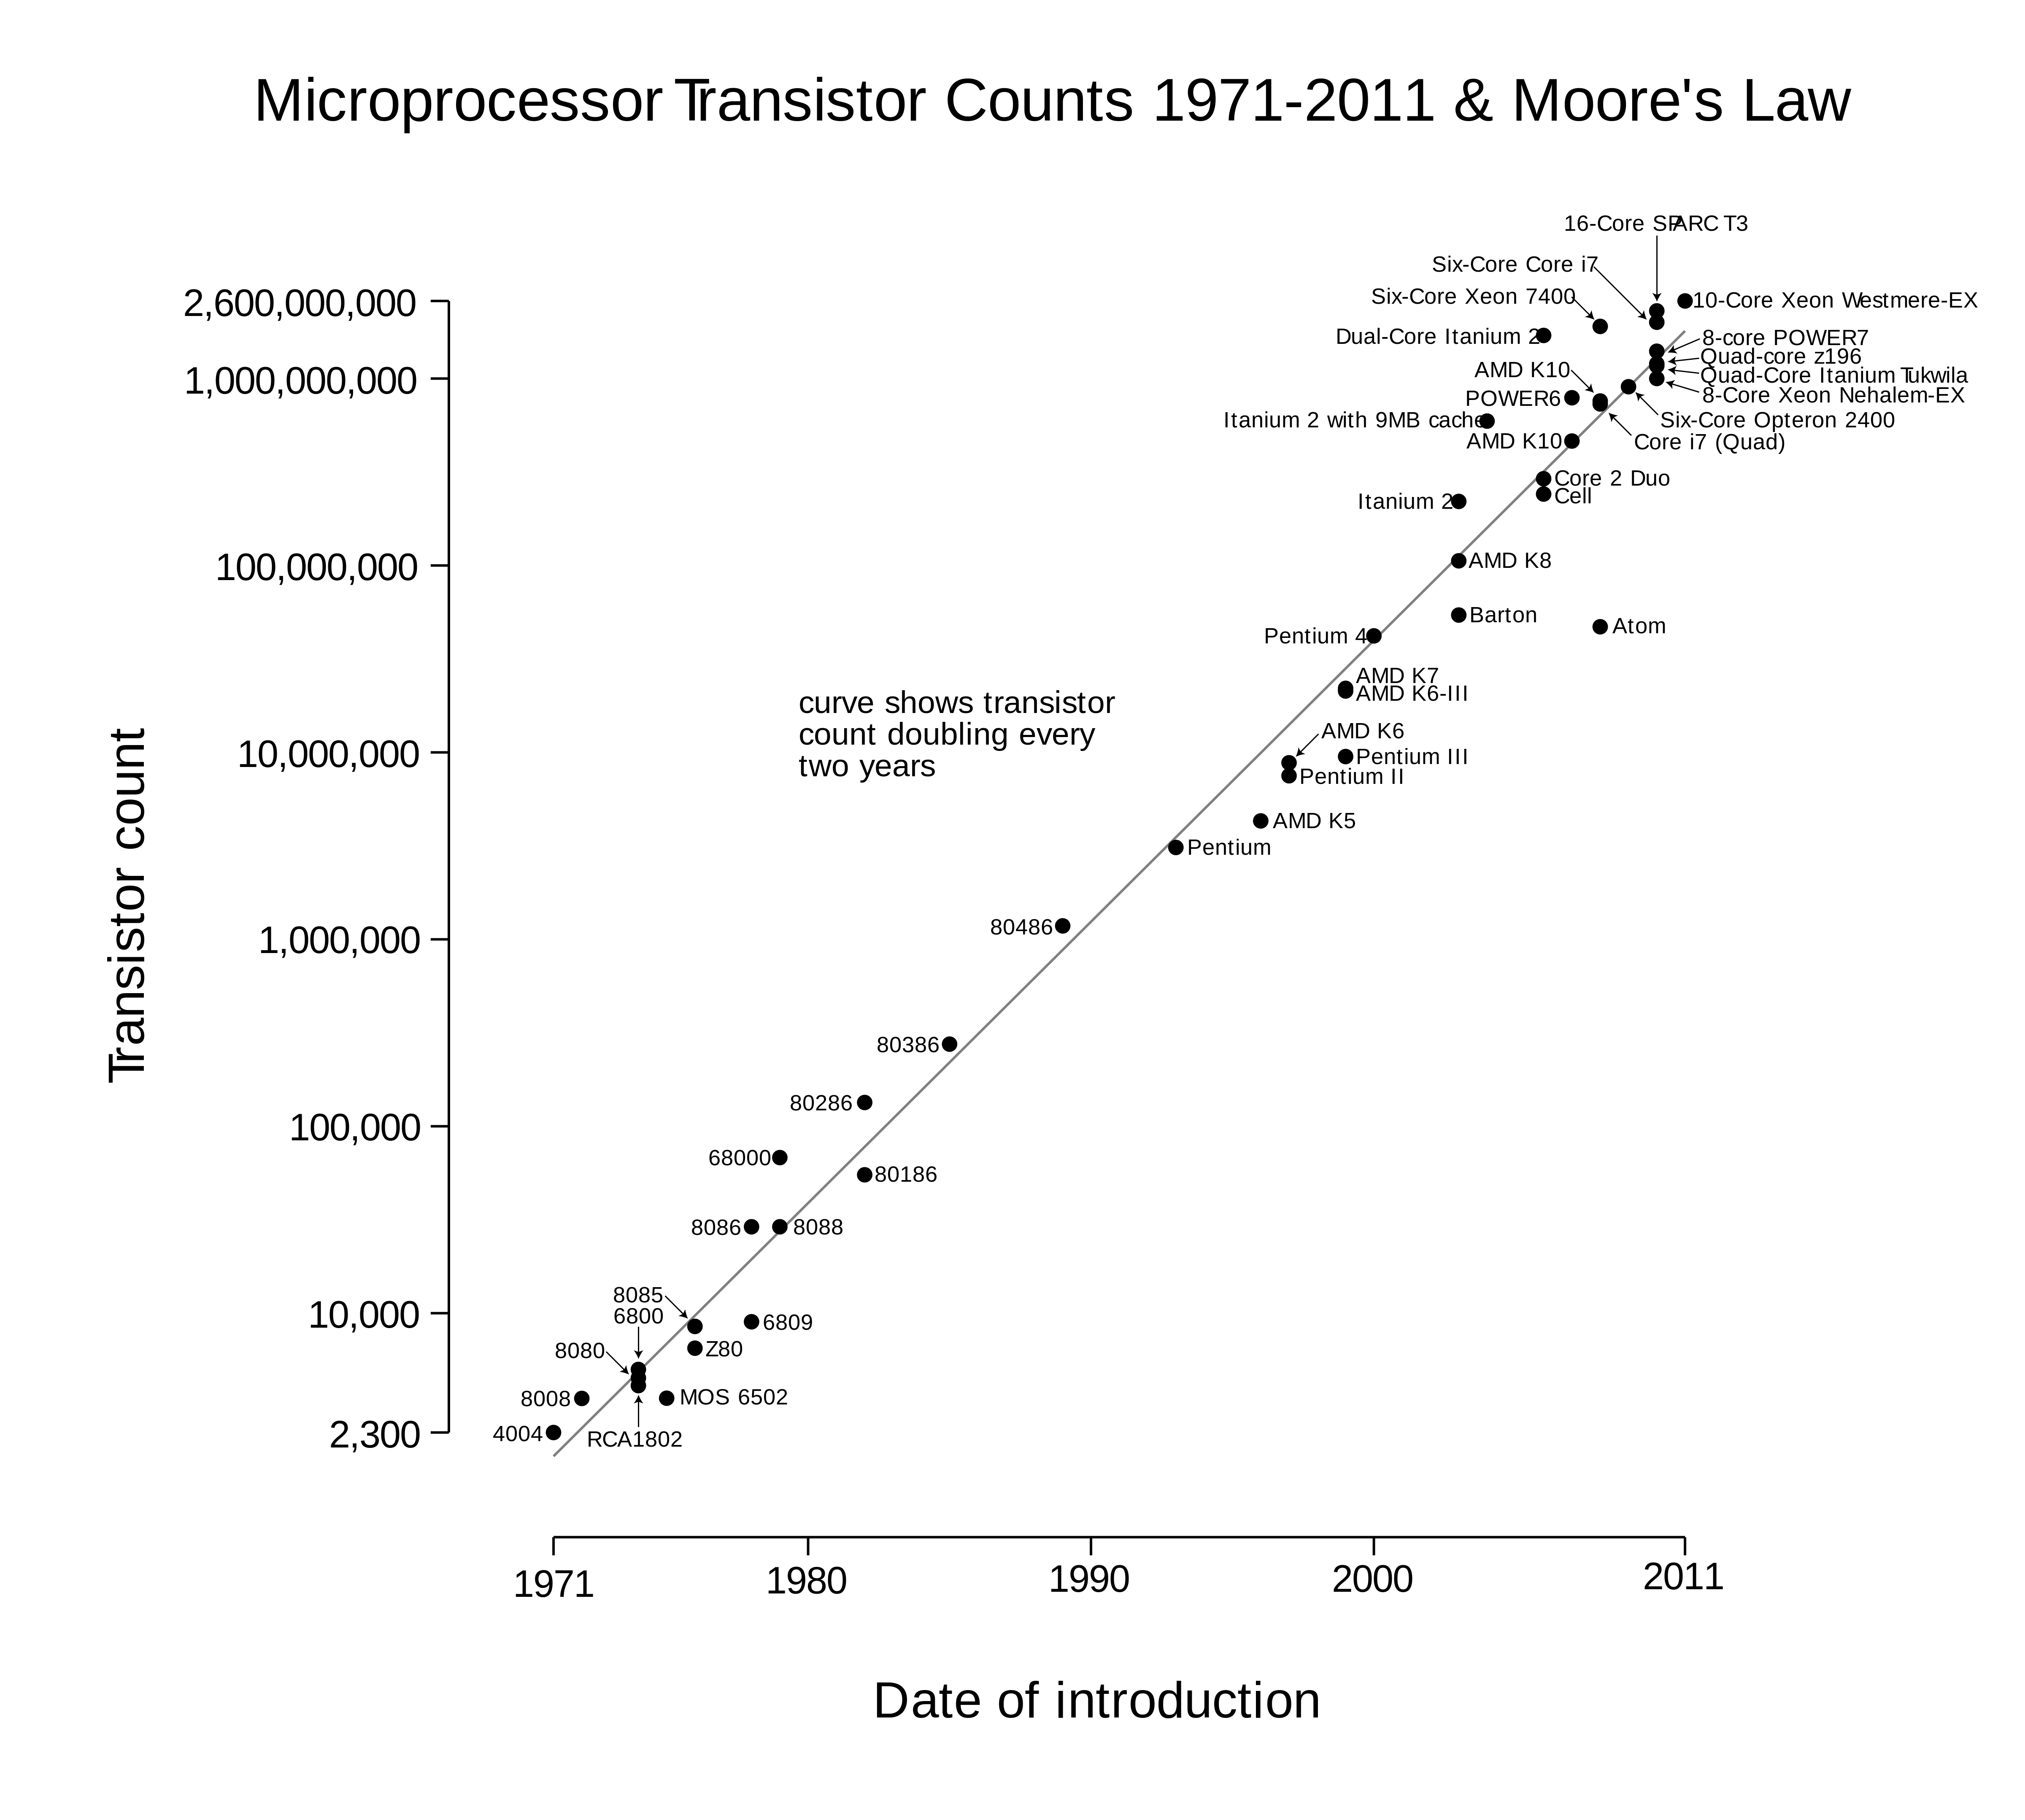
\includegraphics[width=\textwidth,scale=0.6,keepaspectratio=true]{mooreslaw.jpg}
    \caption{
        Graph showing Moore's Law in action, from \cite{WikipediaEN:ML}. Each data point is a processor.
    }
    \label{fig:moore's law}
\end{figure}
Moore's law, which observes that the number of transistors present in an integrated circuit approximately doubles every two years, still stands valid. Processors, and hence computers, have grown faster and faster over years. More and more transistors meant the processors could run faster, at a faster frequency. Processors with better and better clock speeds were introduced every year since the 1980s until around 2004 when instead of single core processors running at faster clock speeds, multi-core processors started rolling out.
\subsection{Why Parallelization?}
\begin{figure}[h]
    \centering
    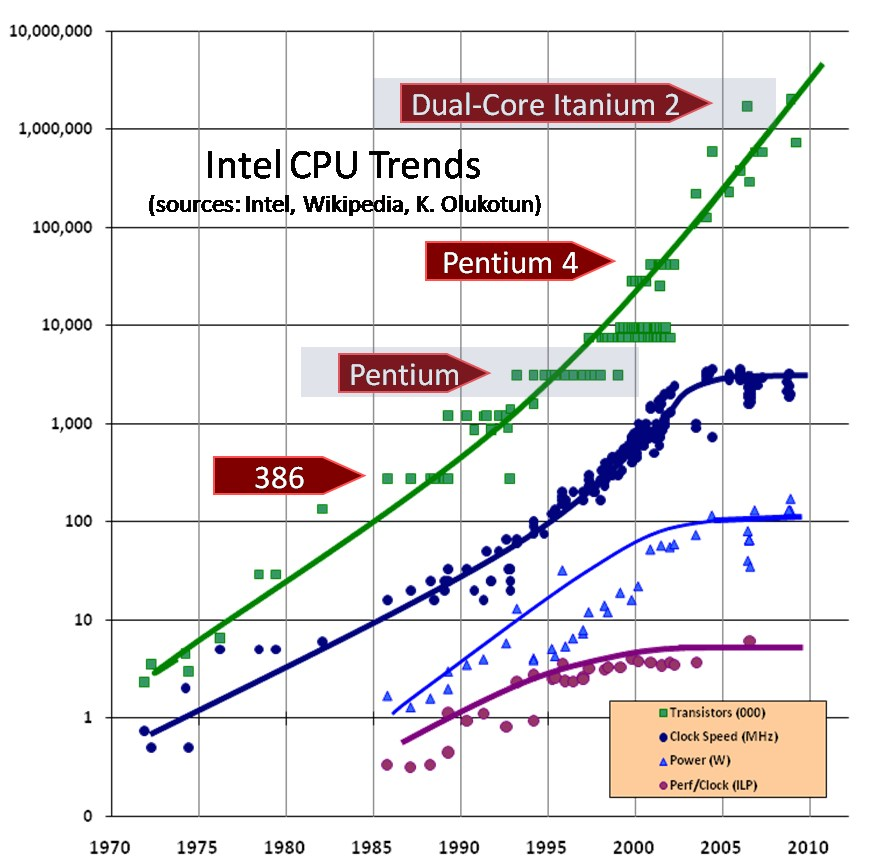
\includegraphics[width=\textwidth,scale=0.6,keepaspectratio=true]{CPU-Scaling.jpg}
    \caption{
        \textit{Intel}'s transition from single core processors to multi-core processors around 2004-2005, from \cite{Herb:Intel}.
    }
    \label{fig:intel}
\end{figure}
Around 2004, Intel and other processor manufacturing companies came to realize that frequency scaling was not practical anymore. The increase in frequency meant an increase in power consumption which inturn meant an increase in heat generation. Thus it was no longer practical to increase the clock speeds of processors. Rather, they started making processors with the same clock speeds, but with multiple cores. Since then the computer architecture industry held fast to the paradigm of multi-core processors. This, in the case of \textit{Intel}, is indicated in the figure \ref{fig:intel}.

Parallelization enables us to run programs faster by splitting the work across different cores of a processor which are ideally run in parallel. In an ideal setup, with \textit{n} cores, we should see a speed up of \textit{n}, which means the running time will become $1/n^{th}$ compared to the running time when run on a single core processor. Though we never really reach this ideal speedup, as stated by Amdahl's law etc., we still achieve significant speed ups.
\subsection{Parallezation of Graph Colouring}
Since the computer architecture industry made a shift to the multi-core paradigm, there had to be a shift in programming paradigm to support the newly available parallelism. Almost all the algorithms, programs etc. were designed and developed to run sequentially on a single core processor. Things have changed recently as more and more algorithms and programs are redesigned and redeveloped to make use of the newly availble parallel hardware.

As discussed earlier, Graph Colouring is a computationally complex problem. The existing solutions are either slow or are fast but produce bad colour quality. Also, practical graphs these days are very large with billions of vertices and edges. So, since the advent of parallel programming paradigms, there have been efforts to parallelize this well celebrated graph problem though most of them were meant specifically for distributed computing setups and super computers. In our work, we focus on parallel graph colouring which can be run on parallel hardware available locally. Especially with the advent of GPGPUs, cheap massive parallelism is at a hand's reach.
\section{GPGPU}
In the domain of parallel programs and applications, one big deterrent was that the number of processor cores available for parallelism was small. Most of the multi-core processors have 32 cores at the maximum. Only super computers had a very high number of cores and they came at a price. 
\subsection{Why GPUs?}
Graphics Processing Units, GPUs, have been using parallelism since their birth. They have almost always been very accessible to the normal public as they are much cheaper than super computers. They also came with thousands of cores. But they were specialized for graphics related operations. Then came the paradigm of GPGPU, General Purpose computing on Graphics Processing Units. And with that, it was now possible to run regular operations and not just graphics related operations on the GPU. GPGPU brought with it easy, cheap access to massive parallelism.
\subsection{nVidia CUDA}
nVidia, one of the biggest players in the GPUs market, introduced its famous parallel computing platform, CUDA, in 2006, thus enabling easy GPU based parallel acceleration. In our work, we use CUDA C to parallelize graph colouring. CUDA lets us harness the power of thousands of cores in the CUDA enabled nVidia GPUs.
\subsubsection{Architecture}
\begin{figure}[h]
    \centering
    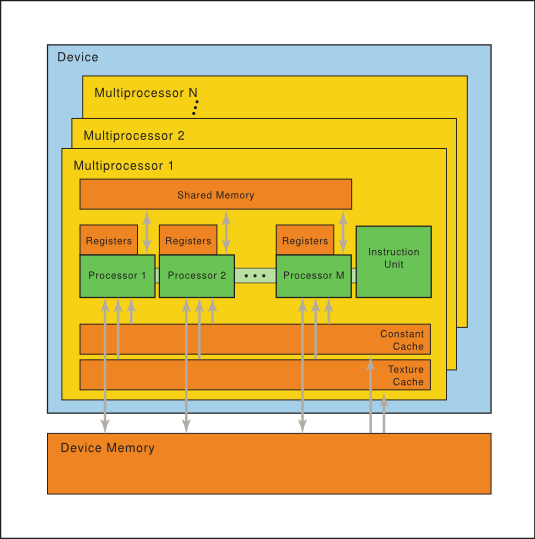
\includegraphics[width=\textwidth,scale=0.4,keepaspectratio=true]{hardware-model.png}
    \caption{
        nVidia GPU hardware model, from \cite{nVidia:Hardware}.
    }
    \label{fig:nvidia}
\end{figure}
In an nVidia GPU, as shown in the figure \ref{fig:nvidia}, there are multiple streaming multi-processors, SMs, and each of these multi processors have thousands of cores/processors in it. Functions to be executed on the GPU are called Kernels and Kernels, once invoked, spawn the required number of threads as blocks of threads which are then executed across SMs. All threads in a block have access to the shared memory inside the SM in which that block is executed.
\subsection{Challenges}
Though, GPUs let us access thousands of threads easily, it comes with a cost. GPU memory and CPU memory are mutually exclusive. So, we have to first copy all the data which are to be processed by the GPU threads to the GPU before invoking the kernels. As the communication between the CPU and the GPU is enabled through the PCI-Express port, which is not super fast, there is a cost for transferring data between the CPU and the GPU. This data transferring cost is one of the biggest overheads in GPU computing. So, as a GPU programmer, one must try to reduce data transfer between the CPU and the GPU.  
\section{Incremental/Decremental}
As we discussed already, Graph Colouring is a very important algorithm on graphs. We have so many practical applications for the same. But most of the practical graphs are dynamic in nature. Vertices and edges are added and deleted often. But the number of these changes are very small compared to the size of the full graph. So, it follows that it is not wise to rerun the graph colouring algorithm on the entire graph every time some vertices/edges are added or deleted. Our work on Incremental/Decremental graph colouring tries to take care of precisely the same.

In our work, we try to re-colour only the relevant parts of the graphs on addition/deletion of edges instead of re-colouring the entire graph. We consider only addition/deletion of edges as deletion of a vertex is considered as the deletion of all edges incident on that vertex. We consider different implications of Incremental/Decremental colouring such as the amount of time we save vs maintaining/improving the colour quality.

\chapter{PARALLEL GRAPH COLOURING}
\chapter{PARALLEL GRAPH COLOURING: INCREMENTAL}
\chapter{PARALLEL GRAPH COLOURING: DECREMENTAL}
\chapter{EXPERIMENTAL EVALUATION}
\section{Experimental Setup}
\section{Test Data}
\section{Parallel Graph Colouring on GPU}
\section{Incremental Parallel Graph Coloruing on GPU}
\section{Decremental Parallel Graph Colouring on GPU}
\chapter{CONCLUSION AND FUTURE WORK}
%%%%%%%%%%%%%%%%%%%%%%%%%%%%%%%%%%%%%%%%%%%%%%%%%%%%%%%%%%%%
% Appendices.

%\appendix
%
%\chapter{A SAMPLE APPENDIX}
%
%Just put in text as you would into any chapter with sections and
%whatnot.  Thats the end of it.

%%%%%%%%%%%%%%%%%%%%%%%%%%%%%%%%%%%%%%%%%%%%%%%%%%%%%%%%%%%%
% Bibliography.
\pagebreak
\begin{singlespace}
  \begin{small}
	\bibliography{refs}
  \end{small}
\end{singlespace}


%%%%%%%%%%%%%%%%%%%%%%%%%%%%%%%%%%%%%%%%%%%%%%%%%%%%%%%%%%%%
% List of papers

%\listofpapers
%
%\begin{enumerate}  
%\item Authors....  \newblock
% Title...
%  \newblock {\em Journal}, Volume,
%  Page, (year).
%\end{enumerate}  

\end{document}
